\documentclass[conference]{IEEEtran}
\IEEEoverridecommandlockouts
% The preceding line is only needed to identify funding in the first footnote. If that is unneeded, please comment it out.
\usepackage{cite}
\usepackage{amsmath,amssymb,amsfonts}
\usepackage{algorithmic}
\usepackage{graphicx}
\usepackage{textcomp}
\usepackage{xcolor}
\usepackage{hyperref}
\usepackage{multicol}
\usepackage{orcidlink}
\usepackage[utf8]{vietnam}
\usepackage{tikz,xcolor,hyperref}

\definecolor{lime}{HTML}{A6CE39}
\DeclareRobustCommand{\orcidicon}{
	
\begin{tikzpicture}
	\draw[lime, fill=lime] (0,0) 
	circle [radius=0.16] 
	node[white] {{\fontfamily{qag}\selectfont \tiny ID}};
	\draw[white, fill=white] (-0.0625,0.095) 
	circle [radius=0.007];
	\end{tikzpicture}
	\hspace{-2mm}
}
\foreach \x in {A, ..., Z}{\expandafter\xdef\csname orcid\x\endcsname{\noexpand\href{https://orcid.org/\csname orcidauthor\x\endcsname}
			{\noexpand\orcidicon}}
}
\newcommand{\orcidauthorA}{0000-0000-0000-0000}
\newcommand{\orcidauthorB}{0009-0004-3101-4840}

\def\BibTeX{{\rm B\kern-.05em{\sc i\kern-.025em b}\kern-.08em
    T\kern-.1667em\lower.7ex\hbox{E}\kern-.125emX}}

\renewcommand\thesection{\Roman{section}}
\renewcommand\thesubsection{\thesection.\arabic{subsection}/}
\begin{document}
\title{Sinh chú thích cho hình ảnh với cơ chế tập trung\\}
\author{\IEEEauthorblockN{Quang-Huy Ngyen\orcidA, Hoai-Phong Le\orcidB}
\IEEEauthorblockA{\textit{Falcuty of Information Technology, University of Science, VNU-HCM} \\
\textit{Vietnam National University, Ho Chi Minh City, Vietnam}\\
20120497@student.hcmus.edu.vn, 20120545@student.hcmus.edu.vn}
}
\maketitle

\begin{abstract}
Image captioning (chú thích hình ảnh tự động) là một bài toán đầy thử thách và có nhiều ứng dụng trong nhiều lĩnh vực khác nhau.
Gần đây, đã có nhiều tiến bộ đáng kể trong chủ đề này nhờ vào những tiến bộ trong học sâu.
Bài nghiên cứu này sẽ đề cập tới quá trình xây dựng một mô hình học sâu theo kiến trúc encoder - decoder với cơ chế Attention có thể sinh chú thích tự động cho hình ảnh và đề ra các giải pháp để cải tiến mô hình.
Chúng tôi cũng sẽ đánh giá các tập dữ liệu huấn luyện và các phương pháp độ đo đánh giá hiệu suất, cũng như một số vấn đề mở rộng và các thách thức chưa được giải quyết xoay quanh vấn đề này.
\end{abstract} 

\begin{IEEEkeywords}
Image Captioning, Deep Learning, Attention
\end{IEEEkeywords}

\section{Dẫn nhập}
Image captioning (chú thích ảnh / sinh mô tả cho ảnh) là một chủ đề thú vị và được được nghiên cứu rộng rãi trong lĩnh vực học máy.
Từ một tấm ảnh đầu vào, mô hình sẽ sinh ra một câu mô tả văn bản về nội dung bên trong bức ảnh.
Chủ đề này có nhiều ứng dụng trong thực tế, bao gồm: hỗ trợ cho người khiếm thị hiểu được nội dung của hình ảnh, cải thiện khả năng tìm kiếm và truy xuất hình ảnh, trợ lý cho các công việc liên quan đến xử lý hình ảnh, và ứng dụng trong nhiều lĩnh vực khác như truyền thông, quảng cáo, y tế... 

Mặc dù không khó để con người có thể mô tả một hình ảnh, tuy nhiên đây là một nhiệm vụ đầy thử thách đối với học máy.
Rất khó để chú thích một bức ảnh hơn là phân loại và nhận dạng các bức ảnh.
Nó yêu cầu máy tính phải nhận ra các vật thể và đặc trưng trong hình ảnh, tìm ra các mối liên hệ giữa chúng và đưa ra mô tả bằng ngôn ngữ tự nhiên.
Bài toán này kết hợp cả hai chủ đề Computer vision (thị giác máy tính) và NLP (xử lý ngôn ngữ tự nhiên).
Để giải quyết vấn đề này, mô hình học sâu với kiến trúc encoder - decoder (mã hóa - giải mã) được ra đời với hai thành phần: Deep convolution neuron network (CNNs) để trích xuất đặc trưng hình ảnh và Recurrent newron network (RNNs) để mô hình hóa ngôn ngữ. Việc áp dụng thêm cơ chế Attention giúp cải thiện hiệu năng và độ chính xác của mô hình.

\begin{figure}[h]
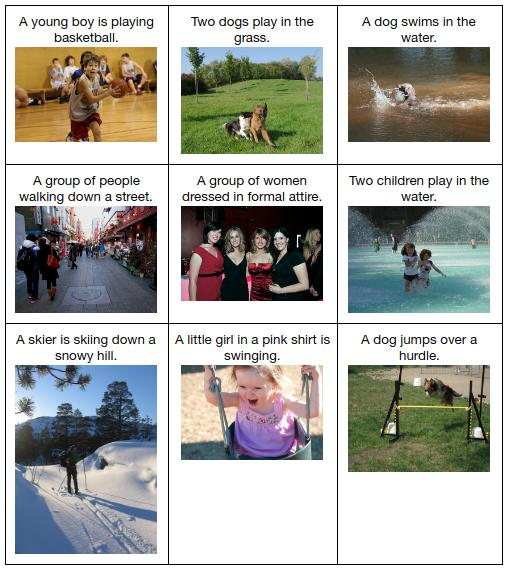
\includegraphics[width=0.5\textwidth]{assets/example.jpg}
  \caption{Ví dụ chú thích cho hình ảnh (câu chú thích sinh ra là tiếng Anh)}
  \label{fig:example}
\end{figure}

\section{Nghiên cứu liên quan}
\subsection{Giải pháp chung}
Những nghiên cứu về Image captioning hầu hết đều sử dụng mô hình học sâu với cấu trúc encoder - decoder khi chúng đã giải quyết vấn đề bằng cách kết hợp hai kĩ thuật về thị giác máy tính và xử lý ngôn ngữ tự nhiên.
Trong cấu trúc encoder - decoder, encoder sẽ trích xuất một vector chứa các feature bên trong ảnh đầu vào và decoder sẽ tạo ra một câu mô tả dựa trên vector chứa các feature tạo bởi encoder.
Encoder thường được dựa trên mô hình CNN và decoder thì dựa trên RNN. Các bài nghiên cứu đều dựa trên việc đề xuất mô hình hoặc cải tiến mô hình bằng các kĩ thuật khác nhau. 

\subsection{Một số kĩ thuật được đề xuất}
\subsubsection{CNNs và LSTMs} 
Mô hình LSTM (Long short-term memory) \cite{hochreiter1997long} là một phiên bản cải tiến của RNN và được dùng phổ biến hơn cho các toán liên quan đến thông tin dạng chuỗi khi nó giải quyết được vấn đề vanishing gradient trong việc xử lý. Ví dụ, Vinyals et al. đã đề xuất mô hình sử dụng CNN cho việc phân loại hình ảnh và LTSM cho việc tạo câu mô tả cho hình ảnh \cite{vinyals2015show} và đã có kết quả có độ chính xác tương đối ổn.
\subsubsection{R-CNNs và LSTM}
Mô hỉnh R-CNNs (Region-based CNNs) được giới thiệu bởi Girshick et al. \cite{girshick2014rich} dùng để giải quyết vấn đề nhận diện object với nhiều tính chất khác nhau (về mặt kích thước, hình dạng,...) khi mà mô hình CNN thông thường sử dụng grid với kích thước cố định. A.K.Yadav đã đề xuất mô hình sử dụng Fast R-CNNs tích hợp VGG-16 cho việc nhận diện vùng và trích xuất đặc trưng và sử dụng mô hình LSTM cho chú thích ảnh. Khuyết điểm của mô hình VGG là lượng tham số lớn và tính toán nặng.  
\subsubsection{ResNet-50 và LSTM}
Mô hình ResNet-50 là một mạng CNN có 50 lớp dùng để giải quyết hiện tượng Vanishing Gradient cũng như tránh tham số quá lớn giúp cho quá trình train diễn ra tốt và nhanh hơn.  Y. Chu \cite{chu2020automatic} đã đề xuất mô hình sử dụng ResNet-50 là một encoder để tạo vector một chiều biểu diễn đặc trưng trong ảnh và sử dụng mô hình LSTM là một decoder để decode vector tạo ra bởi encoder thành một câu chú thích. Đồng thời họ còn sử dụng soft attention ở decoder để có thể tập trung vào một số thành phần trong ảnh để dự đoán được câu tiếp theo tốt hơn. 
\subsubsection{Cơ chế Attention} 
Gần đây, mạng neuron sử dụng cơ chế attention được nghiên cứu, áp dụng cho tác vụ image captioning và tạo ra những đột phá bất ngờ.
Hình ảnh được chia thành các vùng lưới đều và thực hiện tính toán trên từng phần.
Khi RNNs sinh ra những từ mới, cơ chế này sẽ chỉ tập trung vào một số thành phần nhất định có liên quan.
Một ví dụ điển hình là mô hình được đề xuất trong \cite{yan2020image} cho hiệu quả cao hơn mô hình không dùng cơ chế tập trung.


\subsection{Các vấn đề mở rộng}
Có một số nghiên cứu gần đây tiếp cận image captioning theo hướng có thể giải thích được (explainable AI). Do mô hình "hộp đen" của học sâu, các phương pháp cũ không cung cấp đủ manh mối để giải quyết yêu cầu này. Seung-Ho Han et al. \cite{han2020explainable} đã đề xuất một số hướng để tạo một mô hình sinh chú thích ảnh có thể giải thích được.

Một hướng khác là tập trung vào vấn đề cá nhân hóa. Bộ sinh chú thích ảnh sẽ dựa thêm vào các thông tin được cung cấp trước đó về người sử dụng để tạo câu mô tả phù hợp với từng đối tượng người sử dụng khác nhau. Nghiên cứu \cite{chunseong2017attend} đề xuất mô hình Context Sequence Memory Networks để giải quyết vấn đề này.

\section{Phương pháp}
\subsection{Tổng quan mô hình}
Mô hình theo kiến trúc Encoder - Decoder với cơ chế Attention. Trong đó:

a) Encoder: Là mạng neural tích chập (CNN). Có mục đích trích xuất đặc trưng của ảnh đầu vào. Đầu ra của mạng CNN là một vector đặc trưng có kích thước cố định.

b) Cơ chế Attention: Gán trọng số biểu thị mức độ quan trọng cho các đặc trưng hình ảnh. Mô hình sử dụng attention để tập trung vào các vùng quan trọng trong ảnh khi tiến hành tạo chú thích. Cụ thể, mô hình sử dụng cơ chế attention soft để định rõ sự tương quan giữa các đặc trưng của ảnh và từng từ trong chú thích.

c) Decoder: Là mạng neural hồi quy (LSTM). Đầu ra của mạng CNN được sử dụng làm đầu vào cho mạng RNN. Mạng LSTM sẽ sinh ra từng từ trong chú thích dựa trên đầu vào trước đó và các thông tin từ ảnh. 


\subsection{Encoder: CNNs}
Mô hình CNN là mạng neuron truyền thẳng (feedforward neural network), trong đó các lớp được liên kết với nhau bằng phép convolution. Trong đó phép convolution được định nghĩa theo công thức dưới:
$$conv(I,K)_{i,j}=\sum_{a}\sum_{b}\sum_{k}I_{i+a,j+b,k}K_{i,j,k}$$
Trong đó I là ảnh đầu vào nghãi là I là ma trận có kích thước ($n_{H},n_{W},n_{C})$, với $n_{H}$ là chiều cao ảnh, $n_{C}$ số channel, giả sử RGB thì sẽ có $n_{C}=3$, K là filter có kích thước ($n_{f},n_{f},n_{C})$.

Một lớp trong mạng CNN có thể là Convolutional layer, Pooling layer hoặc Fully connected layer. Convolutonal layer là layer chứa các filter tương tự như hidden units và output được tính bằng cách thực hiện phép convolution với đầu vào và sử dụng activation function. Pooling layer được sử dụng để giảm số chiều của ma trận, nhờ đó giảm số tham số để tính cho layer tiếp theo, có 2 loại thường sử dụng là lấy trung bình của một vùng (average) hoặc lấy giá trị lớn nhất trong một vùng (max) với kích thước cho trước. Fully connected layer là một layer chứa các neuron như mạng neuron nhân tạo truyền thống, nhận vào một vector và trả ra vector mới, vì vậy ma trận trước khi đưa vào Fully connected layer sẽ được trải phẳng ra trước, lúc đó vector sẽ có kích thước $n=n_{H}*n_{W}*n_{C}$. Hàm kích hoạt phổ biến nhất cho mạng CNN là hàm ReLU (rectified linear unit), có công thức là:
$$f(x)=max(0,x)$$
giúp cho việc tính toán nhanh hơn và tốc độ hội tụ nhanh hơn. Hình 1 thể hiện một mô hình CNN đơn giản:

\begin{figure}[h]
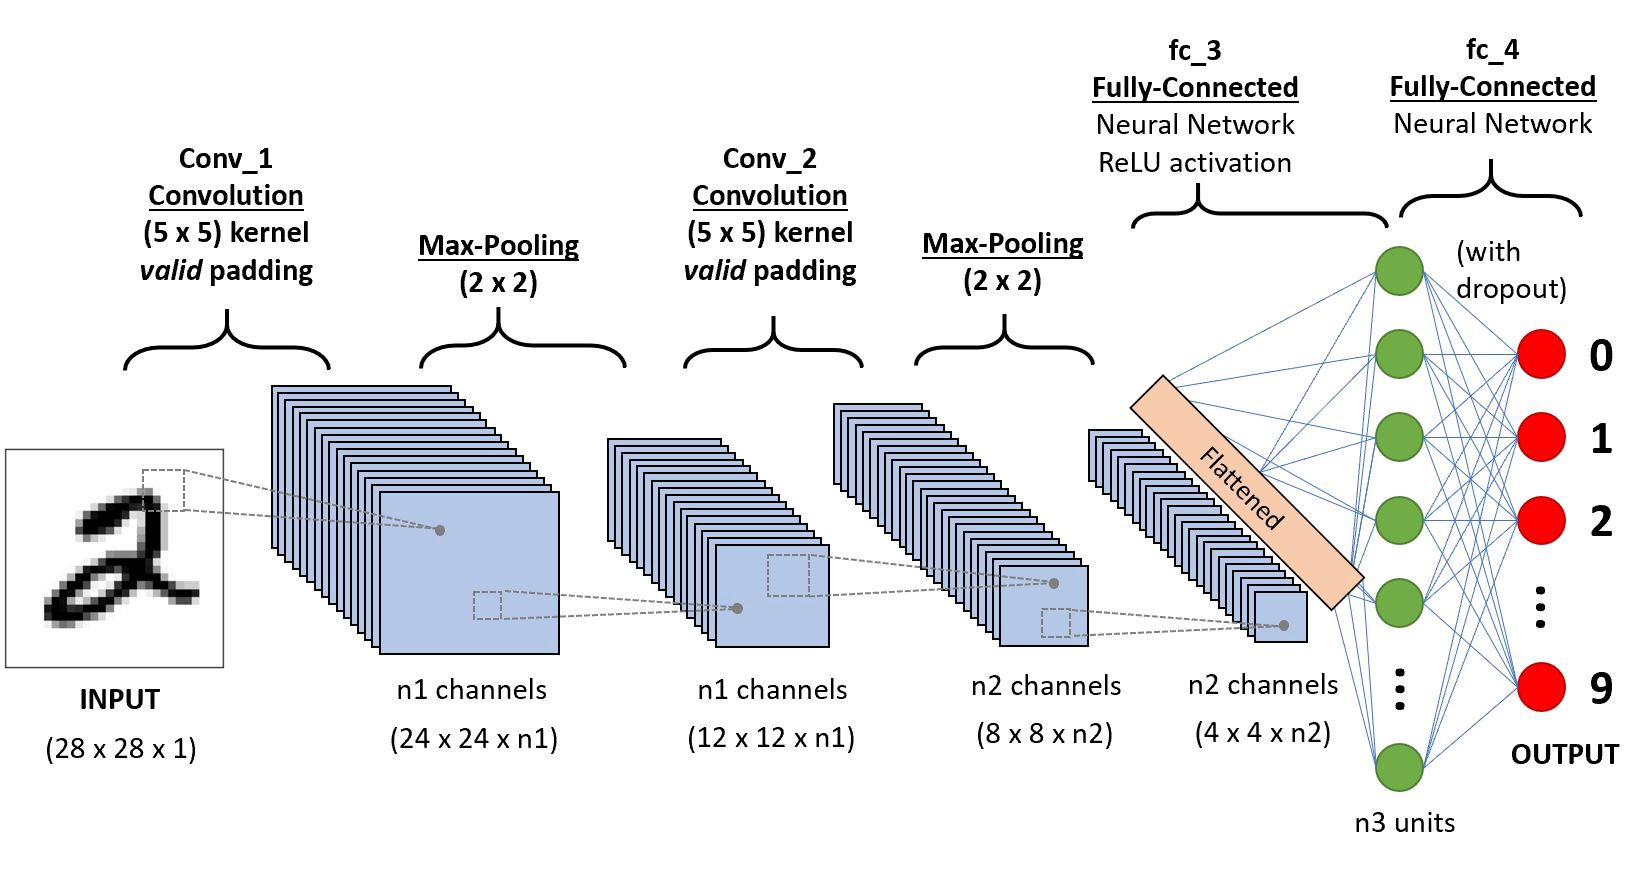
\includegraphics[width=0.5\textwidth]{assets/simpleCNN.jpeg}
  \caption{Minh họa mô hình CNN đơn giản}
  \label{fig:CNN_architecture}
\end{figure}

Trong bài này, nhóm sử dụng một loại mô hình CNN có tên gọi là ResNet-50\cite{he2015deep}. Đây là một mô hình gồm 50 lớp và có thể giải quyết hiện tượng \textit{Vanishing Gradient} khi xây dựng mạng CNN bằng cách sử dụng các \textit{Residual block}, minh họa Residual block so với khối bình thường như ở hình \ref{fig:residual_block}. Với residual block, input có thể lan truyền xuôi (forward propagate) nhanh hơn thông qua cá residual connections (việc đưa input x vào phép tính tổng như hình \ref{fig:residual_block}) ở các layer. Hình \ref{fig:resnet_architecture} thể hiện chi tiết kiến trúc của mô hình ResNet với số layer tương ứng \cite{he2015deep}.

\begin{figure*}[h]
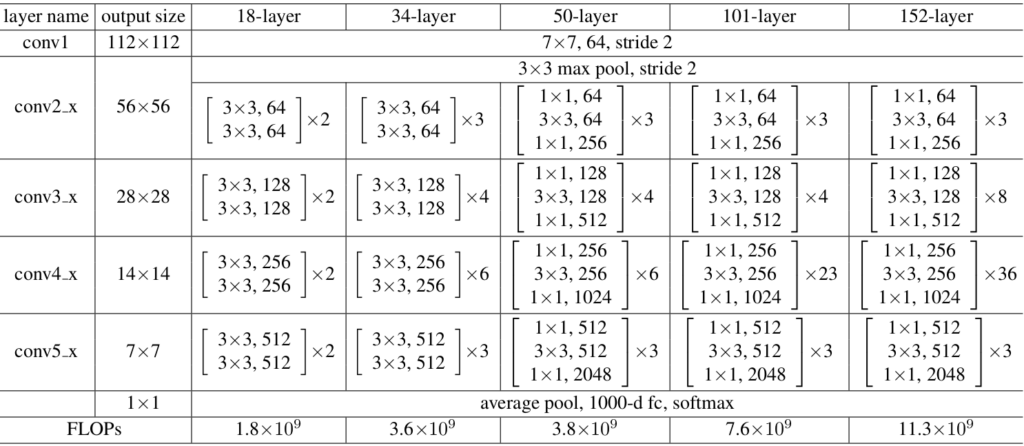
\includegraphics[width=\textwidth]{assets/resnet.png}
  \caption{Kiến trúc của mô hình ResNet với số layer tương ứng }
  \label{fig:resnet_architecture}
\end{figure*}

\begin{figure}[h]
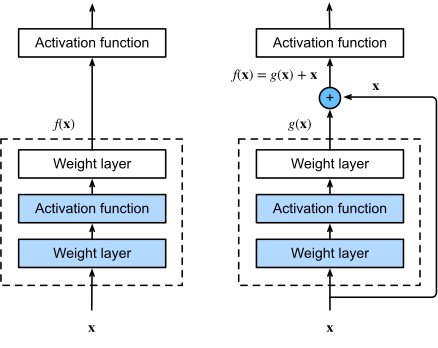
\includegraphics[width=0.5\textwidth]{assets/residual-block.png}
  \caption{Block bình thường (trái) và residual block (phải) }
  \label{fig:residual_block}
\end{figure}



Mô hình này sẽ tạo ra một tập hợp các vector thể hiện đặc trưng, cụ thể là L vector và với mỗi vector thuộc không gian $R^D$ thể hiện các phần trong ảnh. Để có thể trích xuất được vector đặc trưng từ layer, mô hình CNN sẽ bị bỏ bớt các Fully connected layer vì đây là những layer sử dụng để phân loại. 


\subsection{Decoder: LSTMs}
Nhiệm vụ của bộ giải mã là dựa vào ảnh đã được mã hóa và sinh ra câu chú thích theo từng từ.
Các từ được sinh ra dựa vào các vector đặc trưng và cả những từ phía trước nó.
Mạng hồi quy (Recurrent Neural Network - RNN) là một dạng mạng nơ-ron phù hợp để xử lý dữ liệu chuỗi hoặc tuần tự.
Mạng RNN có khả năng xử lý thông tin từ quá khứ và sử dụng nó để tạo ra dự đoán cho các đầu ra trong tương lai.
Điều này rất hữu ích trong việc mô hình hóa các chuỗi dữ liệu có tính tuần tự như ngôn ngữ tự nhiên.

\begin{figure}[h]
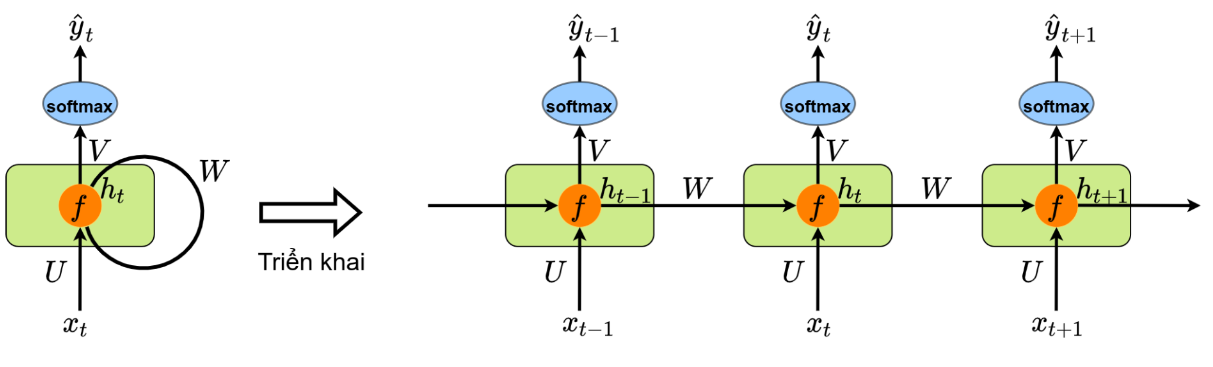
\includegraphics[width=0.5\textwidth]{assets/RNN_model.png}
  \caption{Minh họa kiến trúc RNN}
  \label{fig:RNN_architecture}
\end{figure}

Tuy nhiên RNN gặp vấn đề khi lưu trữ thông tin dài hạn.
Điều này gây khó khăn trong việc huấn luyện mạng và ảnh hưởng đến khả năng của mô hình trong việc ghi nhớ thông tin quan trọng.
Trong quá trình lan truyền ngược mạng RNN, đạo hàm có thể bị bùng nổ hoặc tiêu biến (exploding/vanishing gradient).
Do đó, trong nghiên cứu này, chúng tôi sử dụng biến thể mạnh mẽ của RNN là LSTM\cite{hochreiter1997long} (Long Short-term Memory).

Một đơn vị LSTM có cấu trúc phức tạp hơn đơn vị RNN.'
Nó sử dụng các cổng kiểm soát luồng thông tin (gọi là cổng quên - forgot gate).
Do dó, LSTM có khả năng ghi nhớ thông tin một cách chọn lọc.
LSTM có khả năng ghi nhớ thông tin dài hạn, có khả năng học được các phụ thuộc xa.

Công thức cập nhật trạng thái (cell state) tại thời điểm t trong một đơn vị LSTM được biểu diễn như sau:
$$
\begin{pmatrix}
i \\
f \\
o \\
g
\end{pmatrix}
= 
\begin{pmatrix}
\sigma \\
\sigma \\
\sigma \\
tanh
\end{pmatrix}
\circ
W
\begin{pmatrix}
h_{t-1} \\
x
\end{pmatrix}
$$
$$
c_t = f\circ c_{t-1} + i\circ g
$$
$$
h_t = o \circ tanh(c_t)
$$
$$
p_t = softmax(h_t)
$$

Trong đó, $\sigma$ là hàm sigmoid, i, f, o, g là các cổng quên, với $p_t$ là phân phối xác suất với tất cả các từ. Từ có xác suất lớn nhất được chọn ở từng bước và sẽ được đưa vào bước tiếp theo để tạo thành câu. 

\begin{figure}[h]
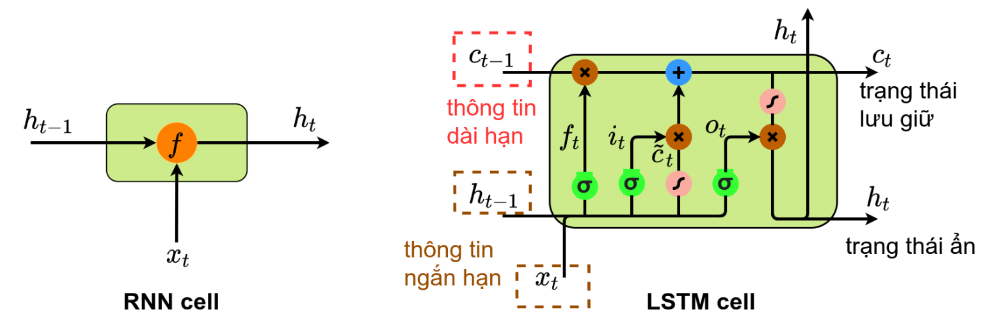
\includegraphics[width=0.5\textwidth]{assets/RNN_LSTM_compare.png}
  \caption{So sánh kiến trúc của đơn vị RNN với đơn vị LSTM}
  \label{fig:RNN_LSTM_compare}
\end{figure}

Trong bài toán image captioning, sử dụng LSTM làm bộ giải mã là lựa chọn phổ biến và hiệu quả.
LSTM cho phép mô hình học các mẫu ngôn ngữ phức tạp, xử lý thông tin từ ảnh và tạo ra các từ dự đoán phù hợp.
Đồng thời, LSTM cũng giúp mô hình duy trì trạng thái ẩn và ghi nhớ thông tin quan trọng từ các từ đã sinh ra trước đó, tạo nên sự liên kết và logic trong câu chú thích.

\begin{figure}[h]
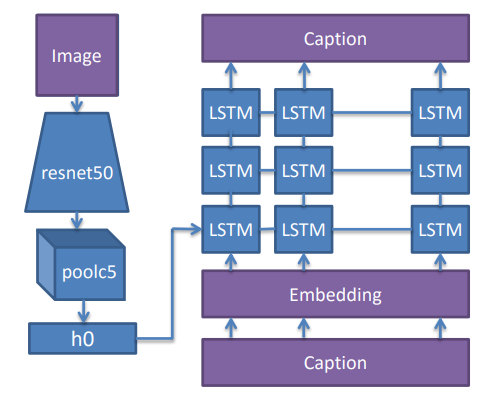
\includegraphics[width=0.5\textwidth]{assets/architecture_CNN_LSTM.png}
  \caption{Minh họa mô hình CNN - LSTM}
  \label{fig:CNN_LSTM}
\end{figure}

\begin{figure}[h]
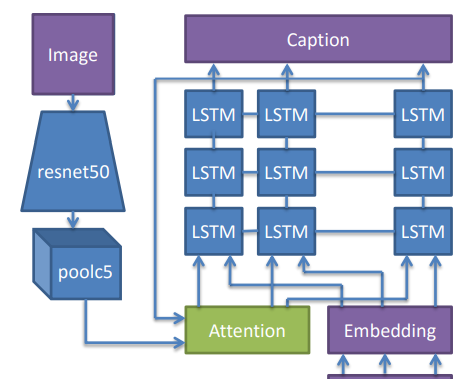
\includegraphics[width=0.5\textwidth]{assets/architecture_CNN_LSTM_attention.png}
  \caption{Minh họa mô hình CNN - LSTM - Attention}
  \label{fig:CNN_LSTM_Attention}
\end{figure}

\subsection{Cơ chế attention}
Hạn chế của mô hình CNN-LSTM hiện tại là thông tin ảnh chỉ được đưa một lần duy nhất tại bước đầu tiên của LSTM, nghĩa là cố gắng decode cả ảnh từ tằng cuối $h_o$.
Ta có thể giải quyết bằng cách đưa toàn bộ thông tin ảnh vào từng bước.
Tuy nhiên, phương pháp này lại gây tốn kém chi phí tính toán.

Một giải pháp tốt hơn là chỉ đưa vào LSTM các phần quan trọng trong ảnh. Để làm điều này, chúng ta có thể sử dụng cơ chế attention mềm (soft attention). Đây là một cơ chế được sử dụng rộng rãi  
để giải quyết các vấn đề về phân loại ảnh. Soft attention được sử dụng bằng cách thêm cổng attention vào LSTM để có thể gán trọng số theo mức độ quan trọng như hình \ref{fig:CNN_LSTM_Attention}. Soft attention phụ thuộc vào kết quả của LTSM ở bước trước đó và đặc trưng đầu vào.  Khi đó, LSTM có công thức cập nhật mới là
$$
\begin{pmatrix}
i \\f \\o \\g \\a_t
\end{pmatrix}
= 
\begin{pmatrix}
\sigma \\ \sigma \\ \sigma \\ tanh \\ softmax
\end{pmatrix}
\circ
W
\begin{pmatrix}
I \circ a_{t-1} \\ h_{t-1} \\ x
\end{pmatrix}
$$
Trong đó: $a_t$ là tham số attention tại thời điểm t. Soft attention là hảm khả vi nên ta có thể sử dụng gradient descent kết hợp backpropagation để huấn luyện. 

\begin{figure}[h]
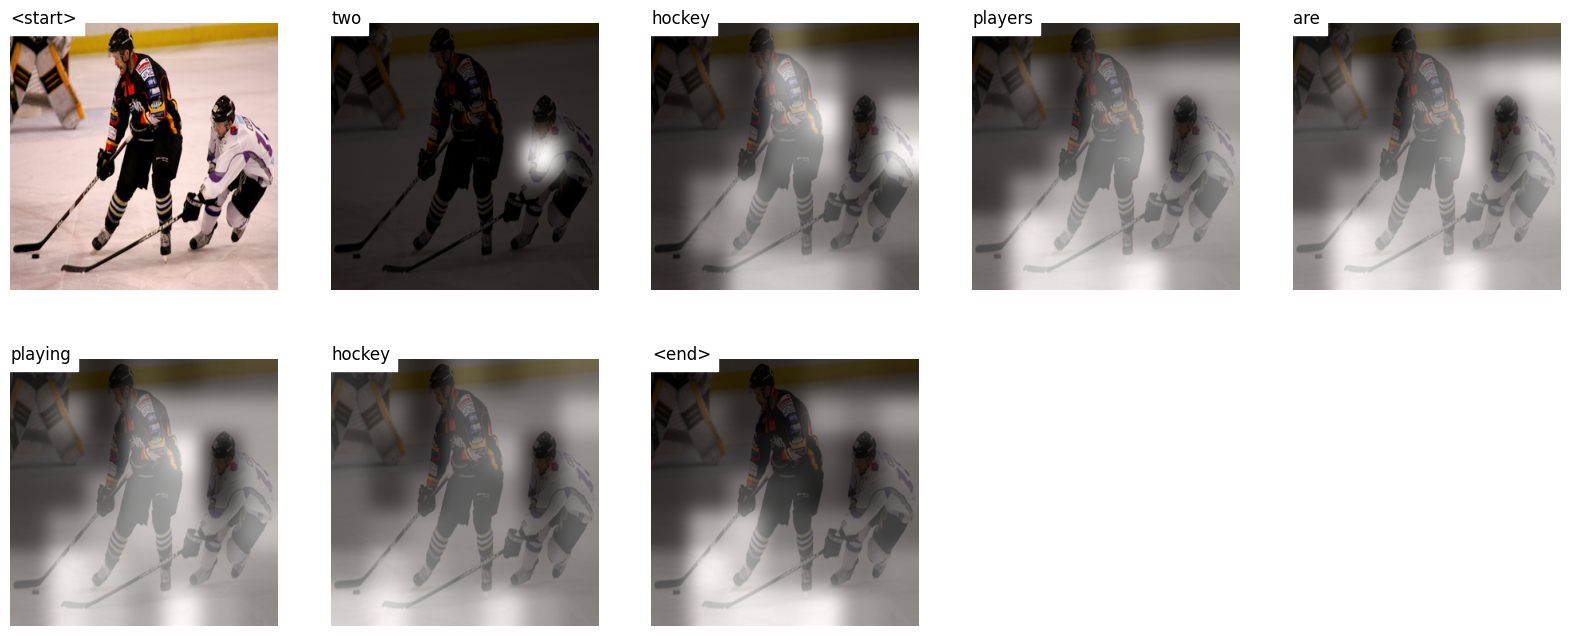
\includegraphics[width=0.5\textwidth]{assets/attention.png}
  \caption{Minh họa vùng ảnh mà mô hình tập trung vào trong quá trình phát sinh câu mô tả. Những vùng ảnh được quan tâm sẽ sáng hơn phần còn lại.}
  \label{fig:RNN_LSTM_attention}
\end{figure}


\section{Thực nghiệm}
\subsection{Tập dữ liệu}
\subsection{Phương pháp đánh giá}
\subsection{Kết quả đánh giá}

\renewcommand{\refname}{Tài liệu tham khảo}
\bibliographystyle{plain}
\bibliography{refs}

\end{document}
